\documentclass[10pt,]{article}
\usepackage{geometry}                % See geometry.pdf to learn the layout options. There are lots.
\geometry{letterpaper}                   % ... or a4paper or a5paper or ... 
\usepackage{graphicx}			% insertar gráficos
\usepackage{amssymb}			% Símbolos
\usepackage{hyperref}			% para incluir hiper-referencias
\usepackage{titlesec}			% Cambiar formato de títulos
\usepackage[plain, noabstract, nocomment]{flexbib} % Para citar con paréntesis y cosas así 
% https://www.nacho-alvarez.es/index.php/blog/2007/04/15/estilo-de-bibliografia-para-bibtex/
% http://www.latex.um.es/retazos/leccion_15/flexbib_manual.pdf
% Editato el spanishbst.tex y flexbib.sty
\usepackage{appendix} % Anexos
\usepackage{subfigure} % Para incluir varias figuras
\usepackage{booktabs}
\usepackage{fontspec,xltxtra,xunicode}		% Por defecto
\defaultfontfeatures{Mapping=tex-text}		% Para usar Century Gothic
\setmainfont[		% Para usar Century Gothic
 BoldFont={Century Gothic Bold}, 
 ItalicFont={Century Gothic Italic},
 BoldItalicFont={Century Gothic Bold Italic}]{Century Gothic}
\usepackage{float} %para usar [H]
\bibpunct{(}{)}{;}{a}{,}{,} % Modificar como se cita https://en.wikibooks.org/wiki/LaTeX/Bibliography_Management

\renewcommand{\bibsection}{\section{Bibliografía\\}} % Cambiar nombre de la bibliografía insertada al final del documento
\renewcommand{\figurename}{Figura} % Cambiar el nombre de las figuras
\renewcommand{\tablename}{Cuadro} % Cambiar el nombre de las tablas
\renewcommand{\contentsname}{Tabla de contenidos\\} % Cambiar el nombre de la tabla de contenidos
\renewcommand{\listfigurename}{Índice de figuras\\} % lista de figuras
\renewcommand{\listtablename}{Índice de cuadros\\} % lista de cuadros
%http://www.elmundoenbits.com/2012/03/latex-problemas-con-el-anexos.html#.WOrWdVKZNE4
\renewcommand{\appendixname}{Anexos}
\renewcommand{\appendixtocname}{Anexos}
\renewcommand{\appendixpagename}{Anexos}


\titleformat*{\section}{\normalsize\bfseries}
\titleformat*{\subsection}{\normalsize\bfseries}
\titleformat*{\subsubsection}{\normalsize\bfseries}

\title{Cuestionario Junta de Vigilancia del Río Elqui y sus Afluentes}
\date{ }                                           % Activate to display a given date or no date

\begin{document}


	\begin{large}
	\begin{center}
		\textbf{Cuestionario Junta de Vigilancia del Río Choapa y sus Afluentes}\bigskip
	\end{center}
	\end{large}
	
	
\begin{enumerate}


\end{enumerate}

\newpage

\section{Cuenca del río Elqui}\bigskip

La hoya hidrográfica del río Elqui se ubica aproximadamente entre los paralelos 29° 35' y 30° 20' de latitud sur, con una superficie total aproximada de 9.800 $km^2$. La zona alta de la cuenca  del río Elqui limita al norte con la cuenca del río Huasco, y con la cuenca del río Los Choros en la zona baja; al sur con la cuenca del río Limarí; y la cuenca costera Elqui - Limarí por el Este.\bigskip

Sus precipitaciones se concentran durante la época de otoño e invierno; opuesto a los mayores requerimientos hídricos que ocurren en los meses de primavera y verano.



\begin{figure}[!h]
\begin{center}
\includegraphics[width=\textwidth]{Figuras/CuencaElqui}
\caption{Cuenca del río Elqui.}
\label{etiqueta_figura1}
\end{center}
\end{figure}

		\subsection{Hidrografía}\bigskip
		
		Los principales cauces tributarios al río Elqui son los ríos Turbio y Claro. La cuenca del río Turbio posee una superficie total de 4.196 $km^2$, donde la generación de su cauce.
		
\section{Junta de Vigilancia del Río Elqui y sus Afluentes (JVRE)}\bigskip

		\subsection{Jurisdicción}
		
		\subsection{Estructuras de almacenamiento}\bigskip

			\subsubsection{Embalse La Laguna}

			\subsubsection{Embalse Puclaro}\bigskip

\section{Sistema de distribución de los recursos hídricos}\bigskip

		\subsection{Levantamiento de criterios de operación}
		En un estudio realizado por la consultora RODHOS, donde pretendían simular escenarios del sistema hídrico de la cuenca del río Elqui, la Junta de Vigilancia del Río Elqui y sus Afluentes les proporcionó información sobre los criterios que establecen para el cálculo de desmarque para la temporada. Estos criterios se señalan a continuación:\bigskip
		
		\begin{itemize}
		
		\item Altura de nieve caída en la temporada, unto con la de la temporada anterior.
		\item Volumen esperado de escorrentía en Elqui en Algarrobal.
		\item Volumen esperado de escorrentía en el río La Laguna en entrada embalse La Laguna.
		\item Castigo de los volúmenes esperados de escorrentía en función del año anterior respecto al actual.
		
		\end{itemize}
		
		\subsection{Reunión Técnica}
		
		El día 19 de enero de 2018 se realizó una reunión técnica en las dependencias de la Universidad de La Serena, Campus Limarí, Ovalle. En ella, participó el Gerente de la Junta de Vigilancia del Río Elqui,  y sus Afluentes Dagoberto Bettancourt junto con el equipo del laboratorio PROMMRA.
		
		indicó criterios en la toma de decisión en la distribución de las aguas en la cuenca, respecto a distintos escenarios que 
		
		
		\subsection{Selección y jerarquización de criterios de operación}
		\subsection{Validación de criterios de operación}\bigskip

\section{Modelo Hidrológico Base}\bigskip

		\subsection{Descripción del modelo Elqui}
		\subsection{Actualización del modelo Elqui}\bigskip
		
			\subsubsection{Incorporación Regla Operacional JVRE}\bigskip
			
		\subsection{Calibración y Validación del modelo Elqui}
		

La Junta de Vigilancia del Río Elqui y sus Afluentes (JVRE), tiene desde el siglo pasado dividido el sistema en tres secciones.\bigskip

La \textbf {Primera Sección} corresponde a los canales pertenecientes a los principales afluentes del río Elqui, es decir, los río Turbio y Claro, y aquellos del propio río desde su formación hasta unos 3 kilometros aguas abajo de la ciudad de Vicuña, donde se ubica el Canal Los Romeros, último de la primera sección. En la actualidad, aunque legalmente no hay cambio oficial de nombre, al hablarse de "Primera Sección", se hace referencia sólo al río Equi, designándose el resto por el río que las sirve (Río Cochiguaz, Río Claro, Río Turbio).\bigskip

La \textbf {Segunda Sección} comprende el río Elqui desde el último canal de la Primera Sección hasta la gran zona de recuperaciones del valle, ubicada al llegar al pueblo de Marquesa. El último canal de esta sección es el canal Quiscal.\bigskip

La \textbf {Tercera Sección}, completa la jurisdicción de la JVRE. Esta comienza muy poco aguas abajo de la bocatoma del canal Casuto, luego de la cual se inicia la seguna y más importante zona de recuperaciones del río. La Tercera Sección termina en la desembocadura del río Elqui al mar.\bigskip

La Junta de Vigilancia ejerce la acción que le otorgan los Estatutos y el Código de Aguas, en toda la hoya hidrográfica del río Elqui y sus Afluentes, incluido el embalse La Laguna, desde la cordillera hasta el mar, con las únicas excepciones del Estero Derecho.\bigskip

Para comprender el sistema de distribución de las aguas del río Elqui y sus afluentes, es necesario definir los conceptos de "río libre" y "río en desmarque", que son de uso común en la zona.\bigskip

Tomando como base que el valor nominal de la acción en el río es de 1 L/s, se entiende como condiciones de "río libre", aquellas en que el valor de la acción alcanza o sobrepasa el valor nominal. Esta es una definición teórica, puesto que en la práctica se declara "río libre" en condiciones menos favorables en cuanto a la disponibilidad hídrica, ya que muchos canales no tienen la capacidad suficiente para captar el gasto con las acciones cotizadas a su valor nominal, o bien los usuarios no desean captarlo por no tener demanda para ser suplida. Expuesto de manera mas sencilla, en las condiciones de "río libre", la Junta de Vigilancia no requiere ejercer control en la toma de los canales, captando cada uno de ellos lo que estime necesario.\bigskip

El ingeniero Juan Bennett, estableció que en promedio por secciones y sectores, es posible declarar "río libre" cuando se cuenta como mínimo, con le caudal necesario para hacer entregas, el cual se muestran en el (Cuadro \ref{my-label})

\begin{table}[H]
\centering
\caption{Desmarque mínimo para considerar "río Libre". (DGA, 1995)}
\label{my-label}
\resizebox{\textwidth}{!}{%
\begin{tabular}{@{}lllllllllllll@{}}
\toprule
\textit{\textbf{Sección}} & \textit{\textbf{May}} & \textit{\textbf{Jun}} & \textit{\textbf{Jul}} & \textit{\textbf{Ago}} & \textit{\textbf{Sep}} & \textit{\textbf{Oct}} & \textit{\textbf{Nov}} & \textit{\textbf{Dic}} & \textit{\textbf{Ene}} & \textit{\textbf{Feb}} & \textit{\textbf{Mar}} & \textit{\textbf{Abr}} \\ \midrule
\textbf{Primera} &  &  &  &  &  &  &  &  &  &  &  &  \\
Claro y Cochiguaz & 25 & 25 & 25 & 25 & 30 & 40 & 45 & 60 & 60 & 50 & 35 & 25 \\
Turbio & 20 & 20 & 20 & 25 & 25 & 35 & 40 & 45 & 45 & 40 & 30 & 25 \\
Vicuña & 30 & 30 & 35 & 40 & 55 & 65 & 70 & 80 & 70 & 65 & 55 & 40 \\
 &  &  &  &  &  &  &  &  &  &  &  &  \\
\textbf{Segunda} & 35 & 35 & 40 & 40 & 45 & 55 & 60 & 55 & 50 & 45 & 40 & 35 \\
 &  &  &  &  &  &  &  &  &  &  &  &  \\
\textbf{Tercera} & 40 & 40 & 40 & 55 & 65 & 90 & 80 & 75 & 70 & 60 & 55 & 45 \\ \bottomrule
\end{tabular}%
}
\end{table}




\begin{itemize}
\item Para realizar interlineado entre párrafos se utiliza \verb!\\!.
\item Para \textbf{escribir en negrita}: \verb!\textbf{texto}!.
\item Para \textit{escribir en cursiva}: \verb!\textbit{texto}!.
\item Para \textit{\textbf{escribir en negrita y cursiva}}: \verb!\textit{\textbf{texto}}! (por lo tanto se pueden anidar los comandos).
\item Para crear una sección: \verb!\section{nombre}!.
\item Para crear una subsección: \verb!\subsection{nombre}!.
\item Para crear una subsubsección: \verb!\subsubsection{nombre}!.
\item Una lista como la actual se crea indicando donde comienza:\\
\verb!\begin{itemize}!\\
Cada ítem se debe ir agregando:\\
\verb!\item! un ítem cualquiera\\
Para cerrar la lista:\\
\verb!\end{itemize}!\\
\item Para cambiar el tamaño de la letra hay muchas opciones, una de ellas es \verb!\scriptsize{texto}! para obtener \scriptsize{un tamaño como este}\normalsize{.} % se bugea el tamaño de texto en listas
\item También se puede escribir en formato máquina de escribir para denotar código u otra cosa que requiera una fuente diferente: \verb!\texttt{texto}! y el \texttt{resultado será así}.
\end{itemize}

Para más información de formato y afines, visitar los sitios web \href{https://es.sharelatex.com/learn}{Share\LaTeX} y \href{https://en.wikibooks.org/wiki/LaTeX}{Wikibooks}.\\

\section{Citas\\}

En el caso de las citas,es algo más complicado de realizar. Primero, hay que descargar e instalar el paquete \texttt{flexbib} para poder personalizar bibliografías en español ya que \LaTeX por defecto compila las bibliografías en inglés (el vínculo de descarga se encuentra en la línea 9 del presente documento). De igual manera de pueden citar los documentos y añadirlos a la bibliografía, pero estarán con el formato en Inglés. Luego, hay que crear una base de datos en Zotero (recomendado) mediante los siguientes pasos:\\

\begin{figure}[!h]
\begin{center}
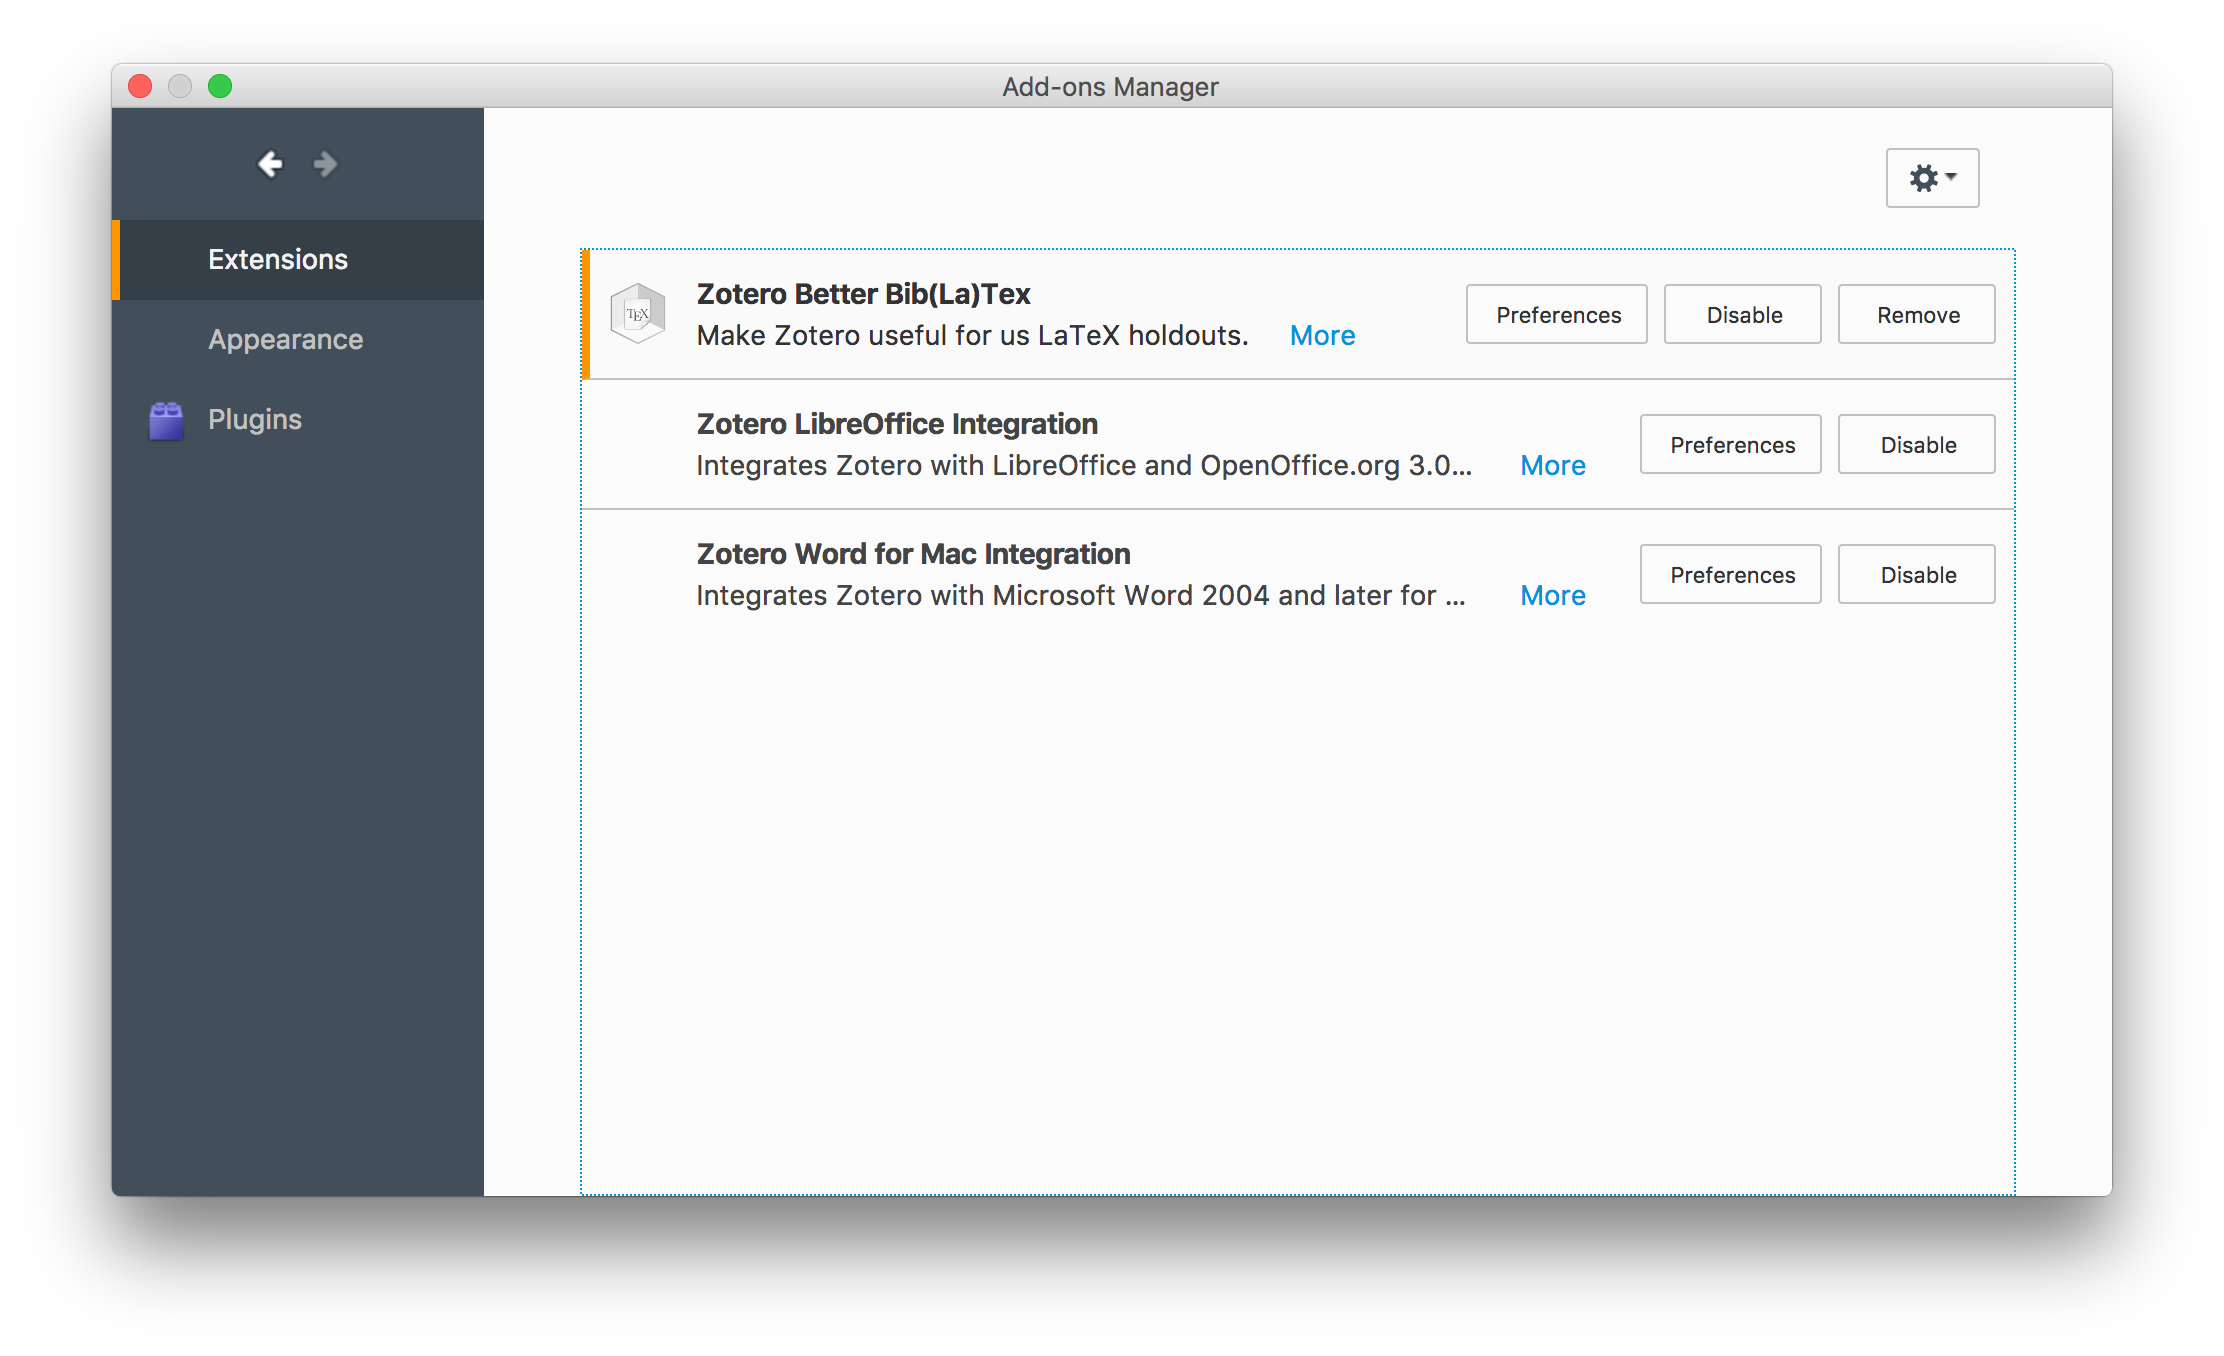
\includegraphics[width=\textwidth]{Figuras/plugins_zotero.png}
\caption{Installar Zotero y los plugins necesarios (especialmente el de flexbib).}
\label{etiqueta_figura1}
\end{center}
\end{figure}

\begin{figure}[!h]
\begin{center}
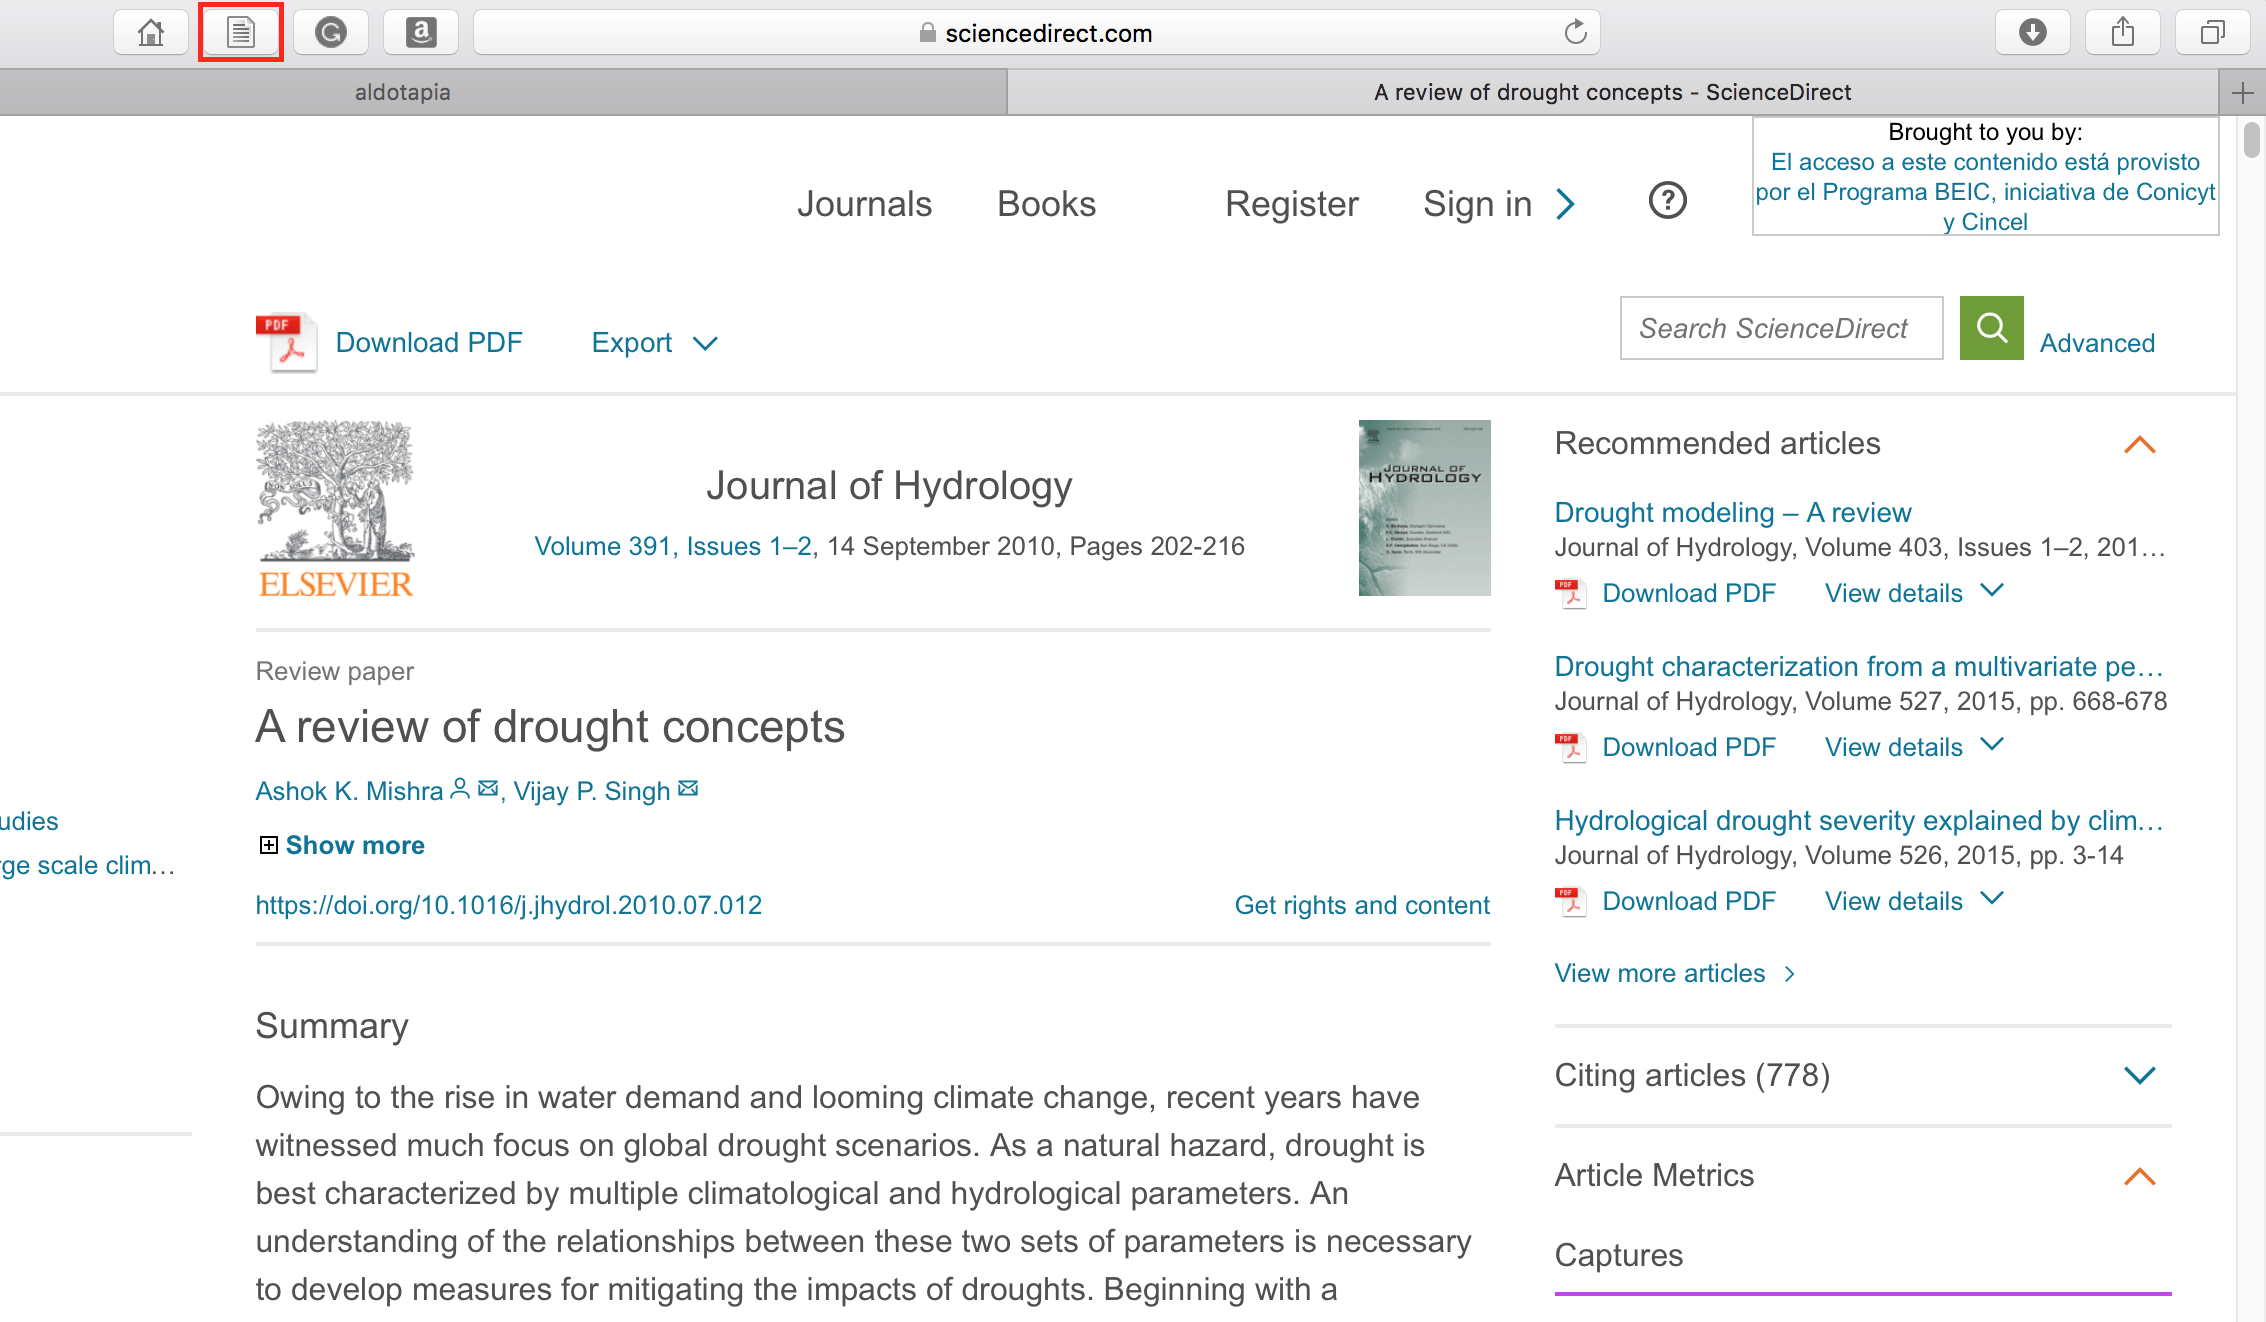
\includegraphics[width=\textwidth]{Figuras/zotero_web.png}
\caption{Clickear el ícono de Zotero para guardar cita}
\label{etiqueta_figura2}
\end{center}
\end{figure}

\begin{figure}[!h]
\begin{center}
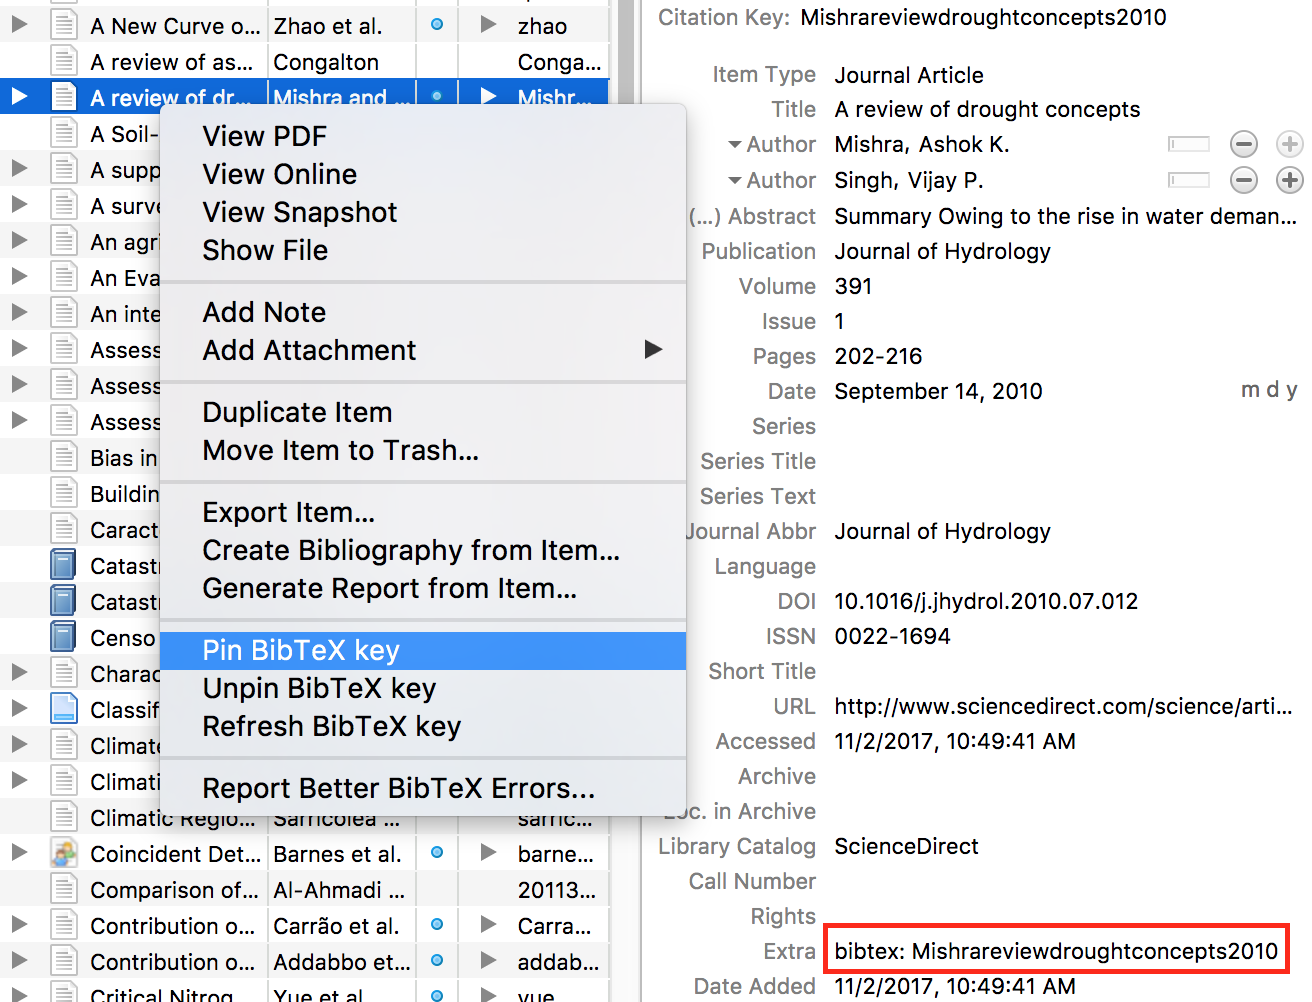
\includegraphics[width=\textwidth]{Figuras/zotero_pin.png}
\caption{Crear un pip de bibtex con la cita}
\label{etiqueta_figura3}
\end{center}
\end{figure}

\begin{figure}[!h]
\begin{center}
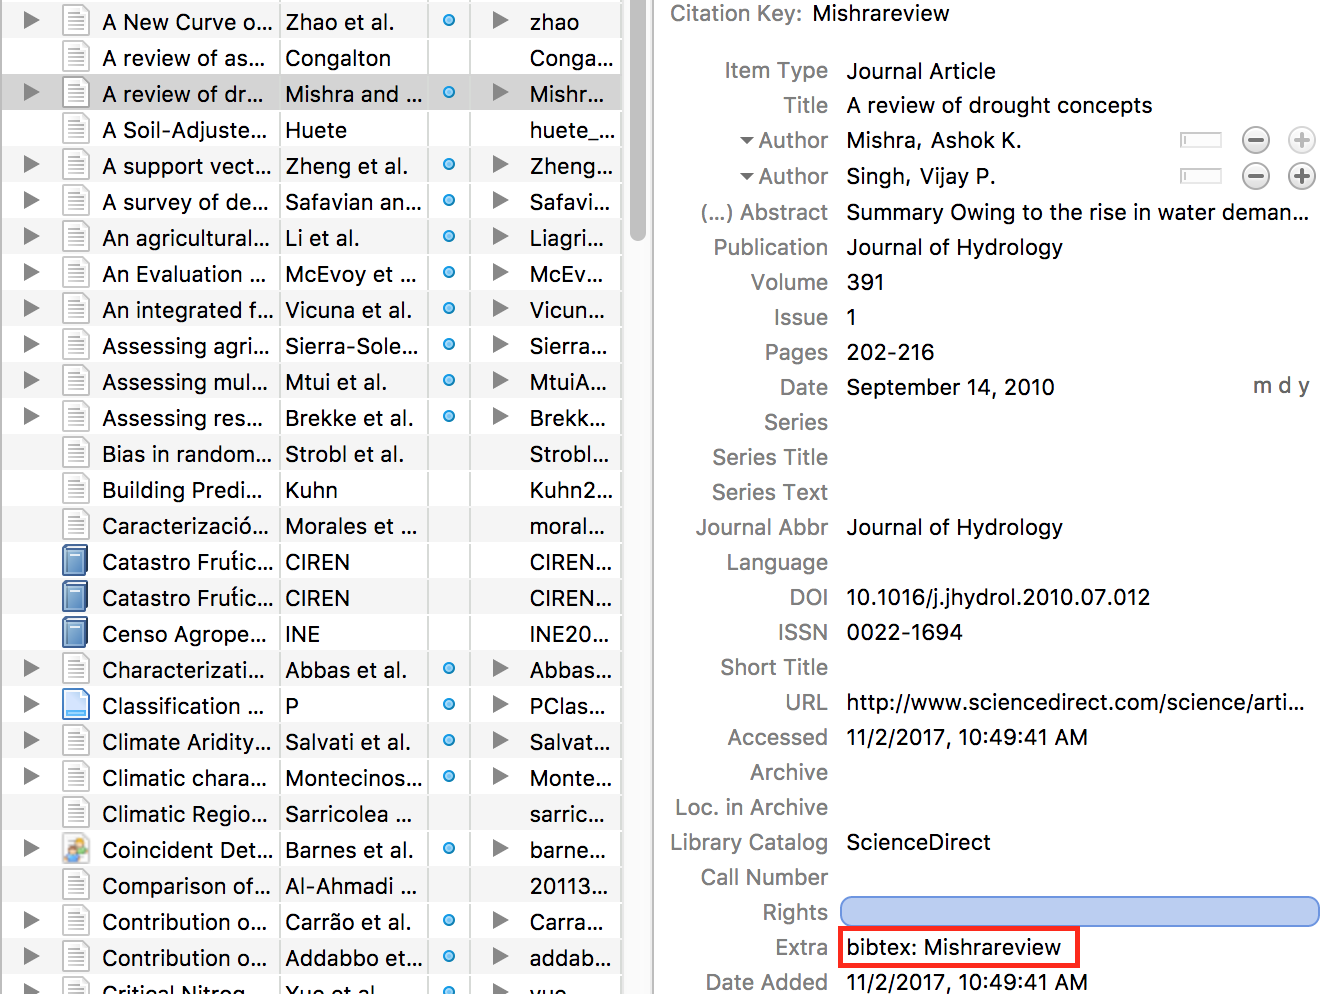
\includegraphics[width=\textwidth]{Figuras/zotero_pin2.png}
\caption{Modificar el pin si se requiere para facilitar la llamada en el documento}
\label{etiqueta_figura4}
\end{center}
\end{figure}

\begin{figure}[!h]
\begin{center}
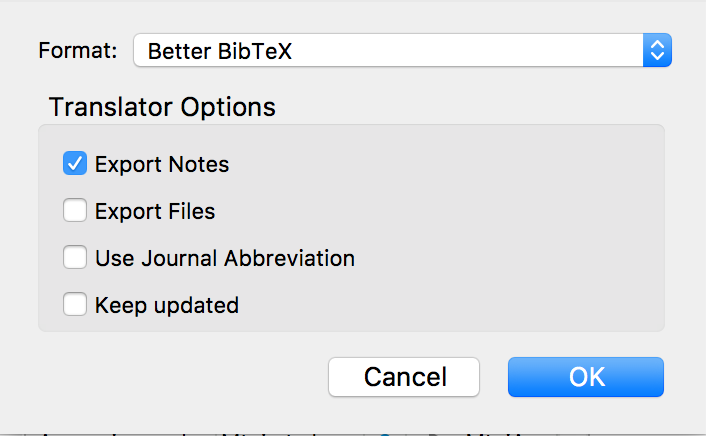
\includegraphics[width=\textwidth]{Figuras/better.png}
\caption{Exportar biblioteca como Better BibTex y guardarla en el mismo lugar donde está almacenado el archivo \texttt{nombre.tex}}
\label{etiqueta_figura5}
\end{center}
\end{figure}

\clearpage

Luego, llamar la cita en base al pin asignado, que en este caso es \verb!Mishrareview! con las funciones \verb!\cite{}! o \verb!\citep{}!. La primera es para citar con mención en el párrafo - como si \cite{Mishrareview} dijo algo - y la segunda; para citar con paréntesis \citep{Mishrareview}. Si se colocan comas entre los corchete para citar a una o más personas - como \verb!\citep{Mishrareview,huete1988}! - el resultado será una cita formateada con separadores \citep{Mishrareview,huete1988}.\\

\subsection{Información importante acerca de las citas\\}

XeLaTeX no compila la bibliografía automáticamente... La elección de este compilador es sólo por el uso de Century Gothic como fuente. Por lo tanto hay que compilar varias primero por XeLaTex, luego por BibTex (para crear la bibliografía), luego nuevamente por XeLaTex (aparecerá la bibliografía, pero las citas estarán con ?) y finalmente una última vez por XeLaTex y todo se compilará a la perfección. Para ello, he ocupado TeXShop para compilar.\\

\textbf{Información importante}: al utilizar RStudio para compilar los documentos, no es necesario seguir los pasos mencionados anteriormente. Sólo se utiliza el ícono \textit{Compile PDF} y el documento quedará correctamente compilado.

\section{Tablas\\}

Lo más sencillo para crear tablas es visitar el sitio web \href{https://www.tablesgenerator.com/latex_tables}{Tables Generator}. Sólo crean la tabla en excel, csv o otro formato. La cargan en el menu desplegable \verb!file! (Figura \ref{tabla1}) y copian el resultado que se obtiene (Figura \ref{tabla2}):

\begin{figure}[!h]
\begin{center}
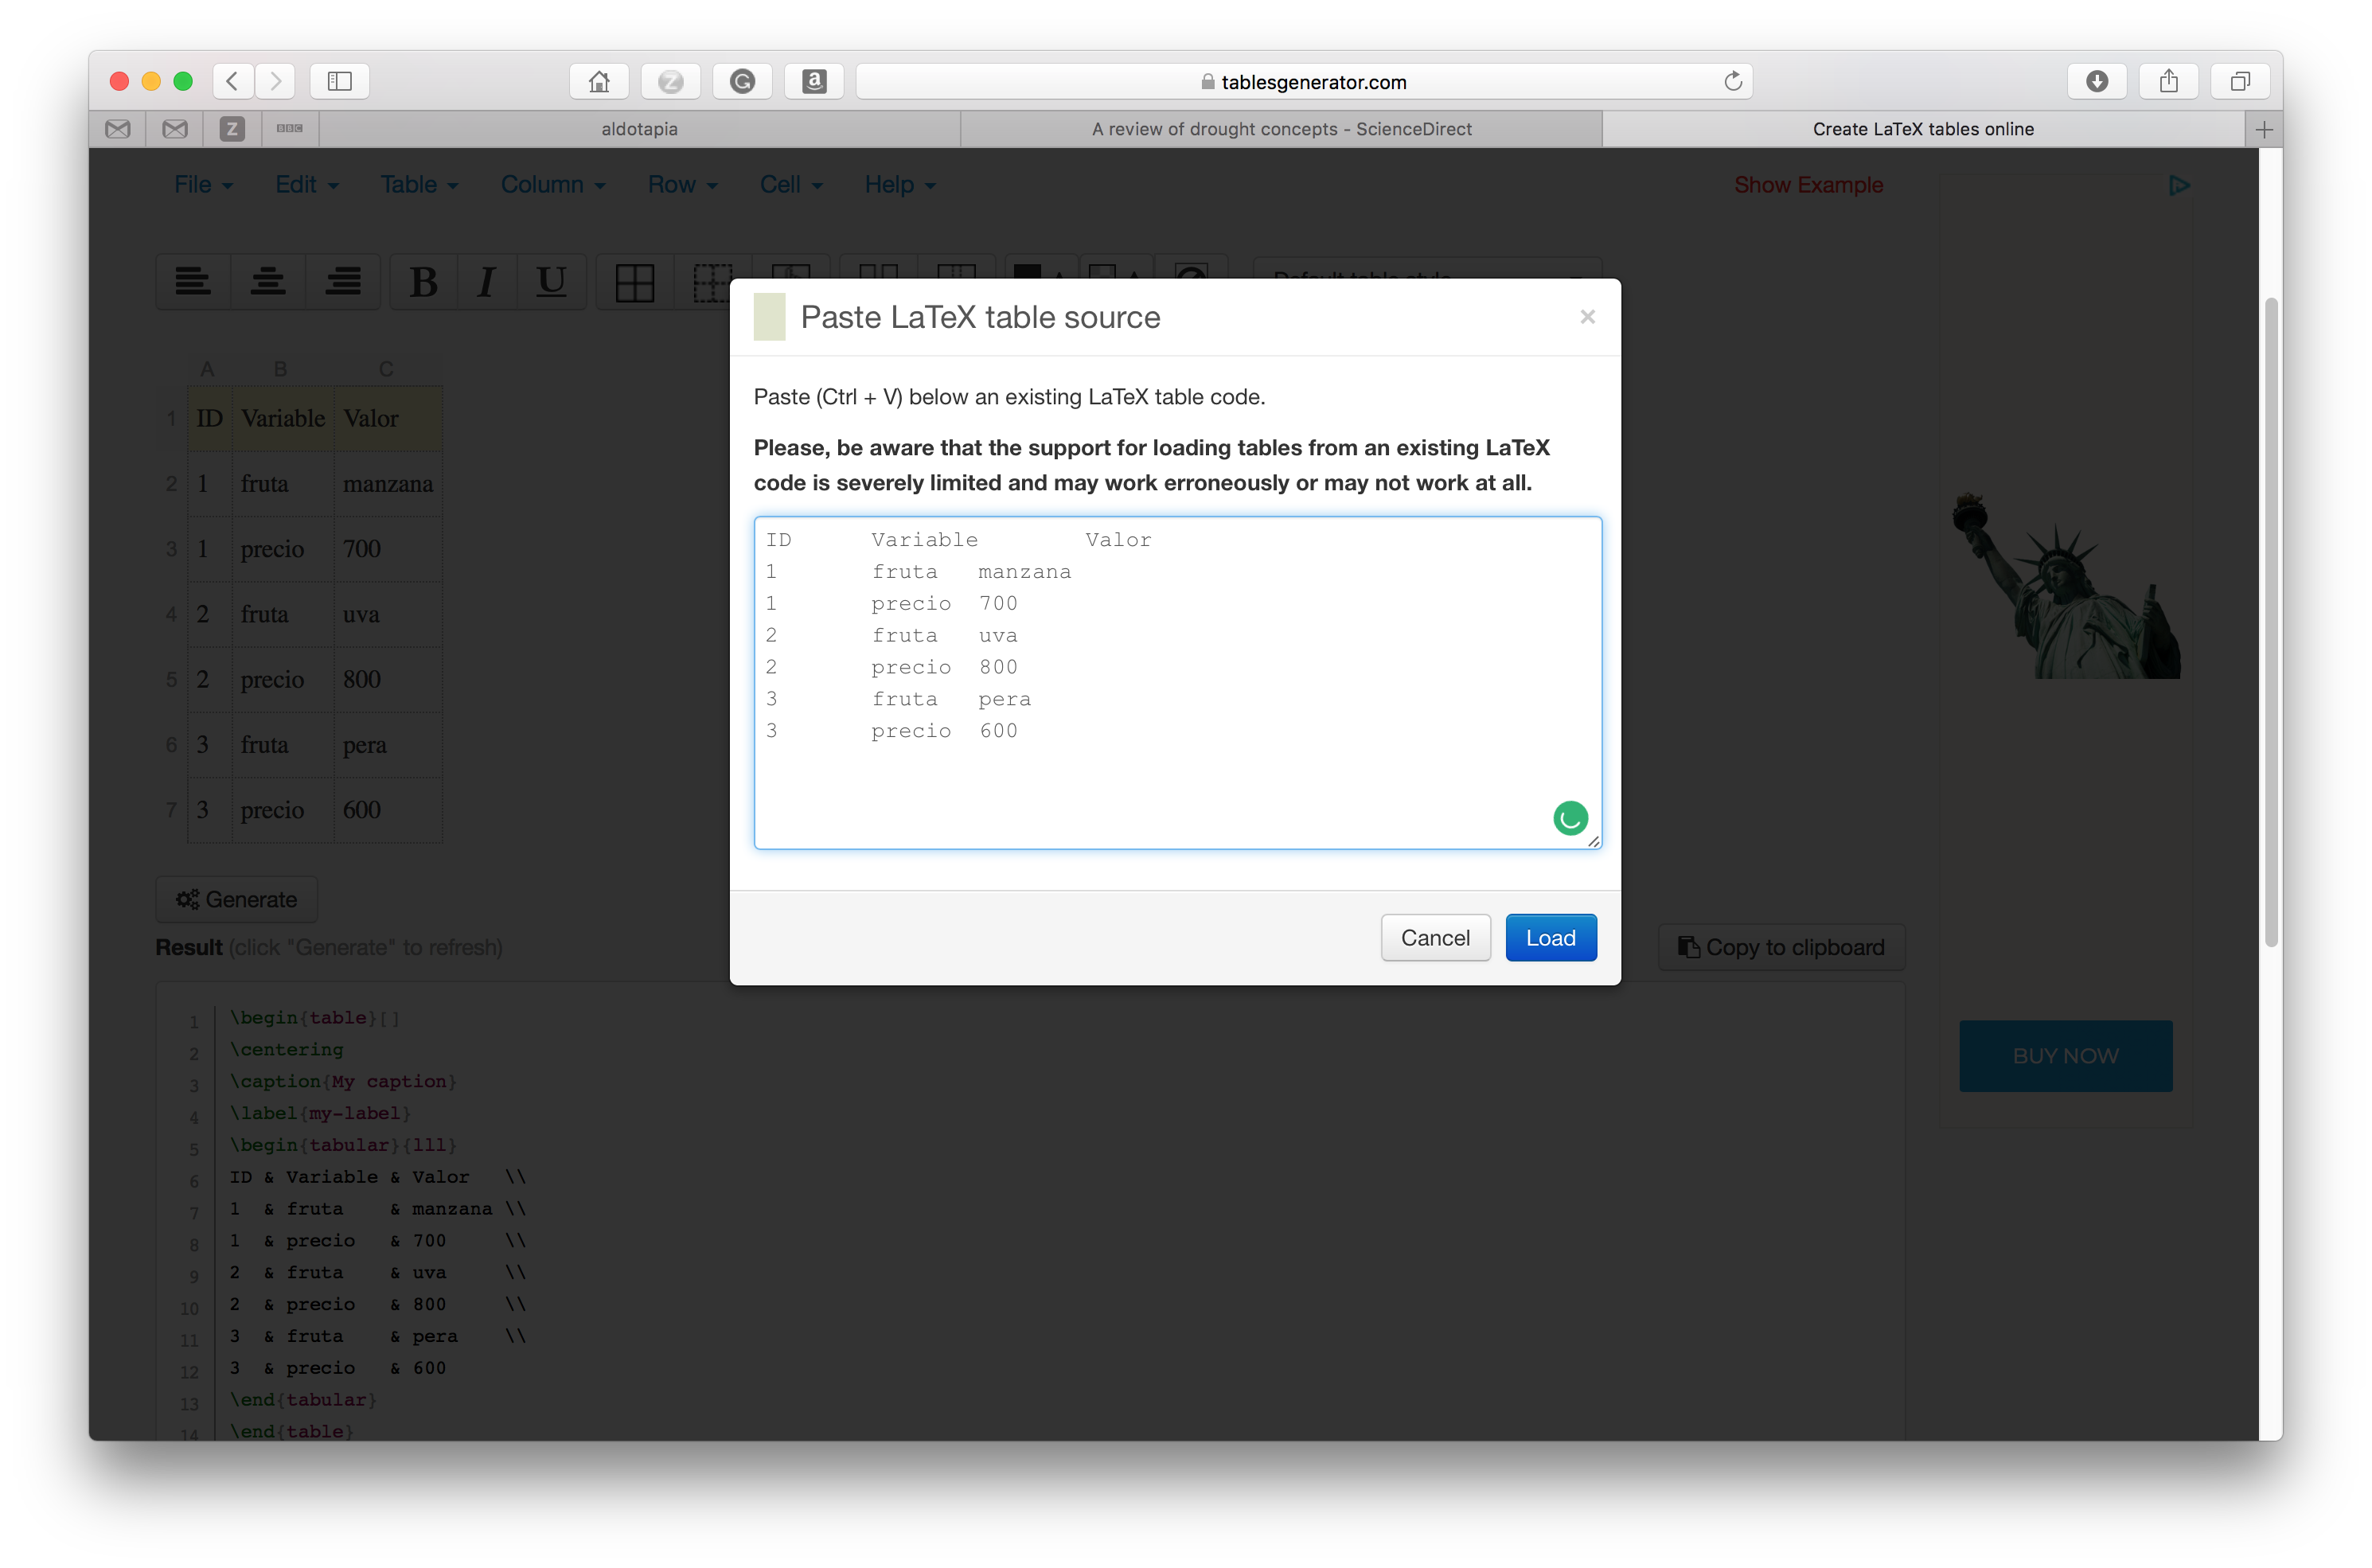
\includegraphics[width=\textwidth]{Figuras/tabla1.png}
\caption{Pegado de la tabla}
\label{tabla1}
\end{center}
\end{figure}

\begin{figure}[!h]
\begin{center}
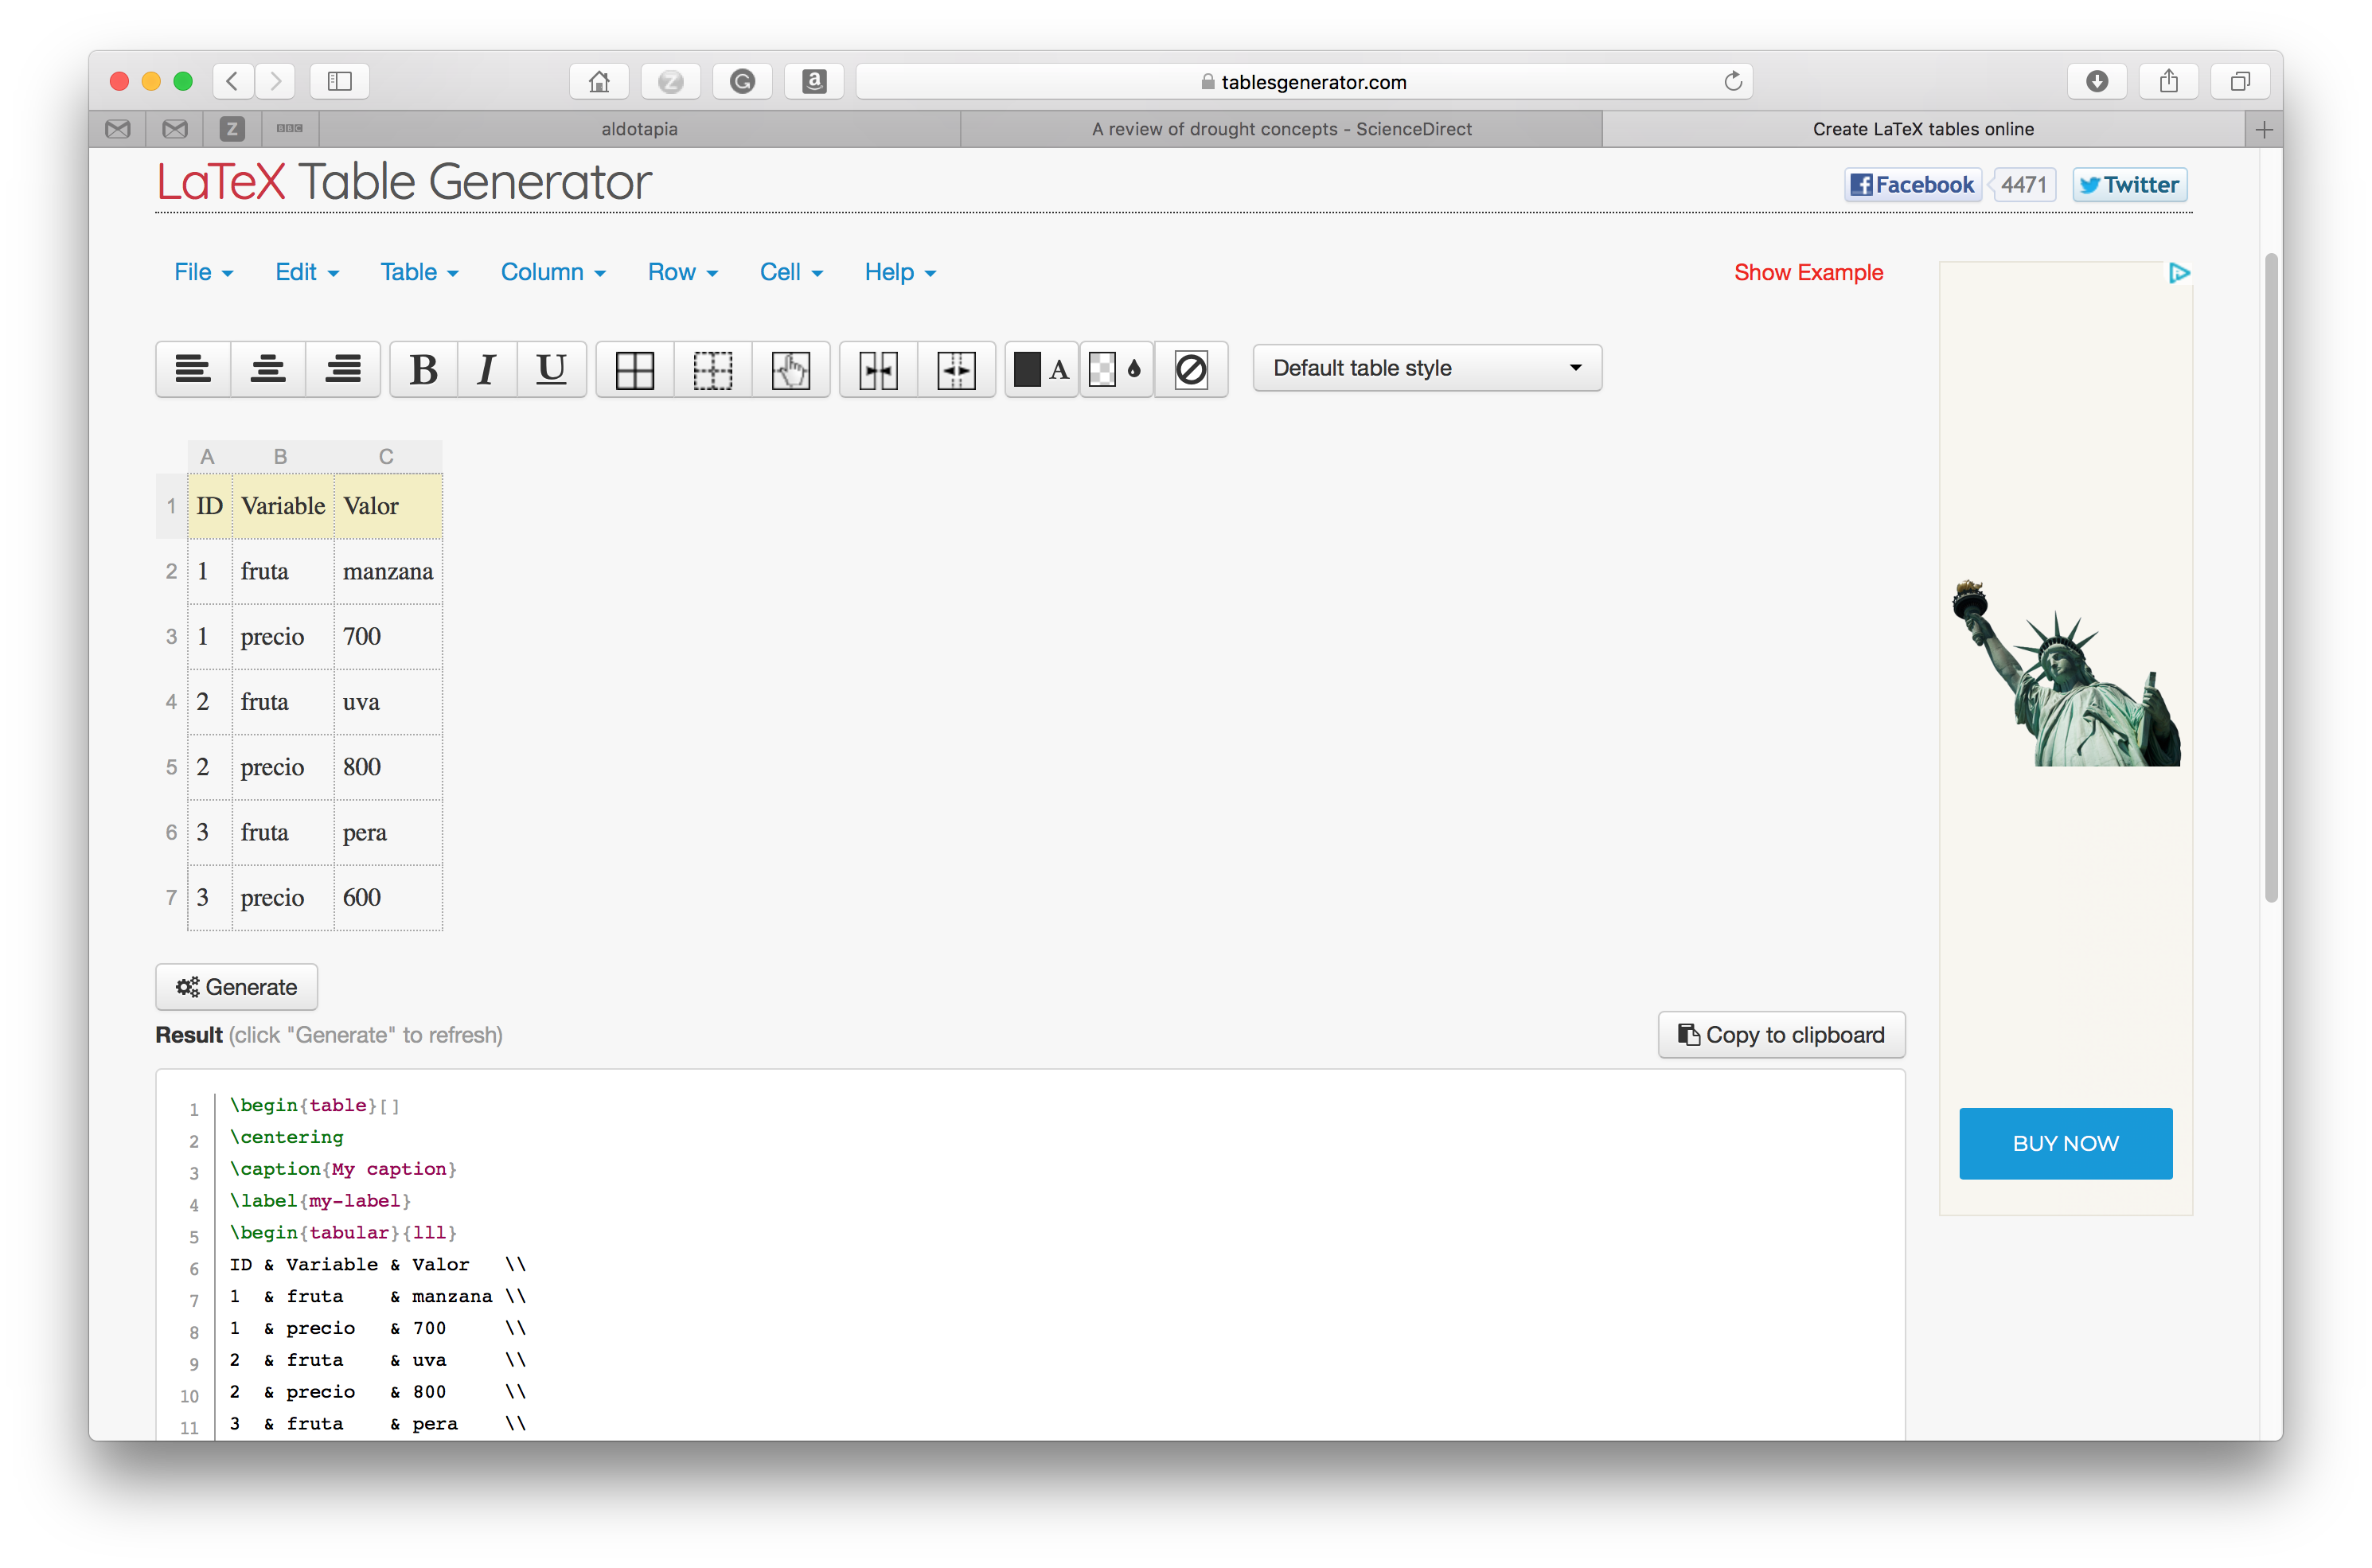
\includegraphics[width=\textwidth]{Figuras/tabla2.png}
\caption{Resultado}
\label{tabla2}
\end{center}
\end{figure}

\clearpage

\begin{table}[]
\centering
\caption{Descripción de la tabla}
\label{etiqueta_tabla}
\begin{tabular}{cll}
ID & Variable & Valor   \\
1  & fruta    & manzana \\
1  & precio   & 700     \\
2  & fruta    & uva     \\
2  & precio   & 800     \\
3  & fruta    & pera    \\
3  & precio   & 600    
\end{tabular}
\end{table}


\bibliographystyle{flexbib}
\bibliography{biblioteca.bib}


\end{document}  